% Options for packages loaded elsewhere
\PassOptionsToPackage{unicode}{hyperref}
\PassOptionsToPackage{hyphens}{url}
\documentclass[
  11pt,
]{article}
\usepackage{xcolor}
\usepackage[margin=1in]{geometry}
\usepackage{amsmath,amssymb}
\setcounter{secnumdepth}{-\maxdimen} % remove section numbering
\usepackage{iftex}
\ifPDFTeX
  \usepackage[T1]{fontenc}
  \usepackage[utf8]{inputenc}
  \usepackage{textcomp} % provide euro and other symbols
\else % if luatex or xetex
  \usepackage{unicode-math} % this also loads fontspec
  \defaultfontfeatures{Scale=MatchLowercase}
  \defaultfontfeatures[\rmfamily]{Ligatures=TeX,Scale=1}
\fi
\usepackage{lmodern}
\ifPDFTeX\else
  % xetex/luatex font selection
\fi
% Use upquote if available, for straight quotes in verbatim environments
\IfFileExists{upquote.sty}{\usepackage{upquote}}{}
\IfFileExists{microtype.sty}{% use microtype if available
  \usepackage[]{microtype}
  \UseMicrotypeSet[protrusion]{basicmath} % disable protrusion for tt fonts
}{}
\makeatletter
\@ifundefined{KOMAClassName}{% if non-KOMA class
  \IfFileExists{parskip.sty}{%
    \usepackage{parskip}
  }{% else
    \setlength{\parindent}{0pt}
    \setlength{\parskip}{6pt plus 2pt minus 1pt}}
}{% if KOMA class
  \KOMAoptions{parskip=half}}
\makeatother
\usepackage{longtable,booktabs,array}
\newcounter{none} % for unnumbered tables
\usepackage{calc} % for calculating minipage widths
% Correct order of tables after \paragraph or \subparagraph
\usepackage{etoolbox}
\makeatletter
\patchcmd\longtable{\par}{\if@noskipsec\mbox{}\fi\par}{}{}
\makeatother
% Allow footnotes in longtable head/foot
\IfFileExists{footnotehyper.sty}{\usepackage{footnotehyper}}{\usepackage{footnote}}
\makesavenoteenv{longtable}
\usepackage{graphicx}
\makeatletter
\newsavebox\pandoc@box
\newcommand*\pandocbounded[1]{% scales image to fit in text height/width
  \sbox\pandoc@box{#1}%
  \Gscale@div\@tempa{\textheight}{\dimexpr\ht\pandoc@box+\dp\pandoc@box\relax}%
  \Gscale@div\@tempb{\linewidth}{\wd\pandoc@box}%
  \ifdim\@tempb\p@<\@tempa\p@\let\@tempa\@tempb\fi% select the smaller of both
  \ifdim\@tempa\p@<\p@\scalebox{\@tempa}{\usebox\pandoc@box}%
  \else\usebox{\pandoc@box}%
  \fi%
}
% Set default figure placement to htbp
\def\fps@figure{htbp}
\makeatother
\setlength{\emergencystretch}{3em} % prevent overfull lines
\providecommand{\tightlist}{%
  \setlength{\itemsep}{0pt}\setlength{\parskip}{0pt}}
\usepackage{bookmark}
\IfFileExists{xurl.sty}{\usepackage{xurl}}{} % add URL line breaks if available
\urlstyle{same}
% fallback for those not using the hyperref driver hyperxmp:
\makeatletter
\@ifundefined{xmpquote}{\newcommand{\xmpquote}[1]{#1}}{}
\makeatother
\hypersetup{
  hidelinks,
  pdfcreator={LaTeX via pandoc}}

\author{}
\date{}

\begin{document}

\section{No alpha-specific transcriptomic signature of the cortical
alpha-rhythm sources targeted by closed-loop EEG--TMS: an
imaging-transcriptomics test of the ENIGMA-EEG oscillatory-power
GWAS}\label{no-alpha-specific-transcriptomic-signature-of-the-cortical-alpha-rhythm-sources-targeted-by-closed-loop-eegtms-an-imaging-transcriptomics-test-of-the-enigma-eeg-oscillatory-power-gwas}

\textbf{Running title:} Alpha genetics and the transcriptomics of
TMS--EEG alpha targets

\begin{center}\rule{0.5\linewidth}{0.5pt}\end{center}

\subsection{Abstract}\label{abstract}

\textbf{Background.} The power and frequency of the
electroencephalographic (EEG) alpha rhythm are among the most heritable
human neurophysiological traits, and a dedicated genome-wide association
study (GWAS) of EEG oscillatory power (ENIGMA-EEG; Smit et al., 2018)
has identified common variants associated with band-limited power. In
parallel, brain-state-dependent EEG--TMS relies on a specific set of
cortical alpha-rhythm sources and their functional-connectivity
architecture (Tabarelli et al., 2022). Whether the genes implicated in
alpha power are transcriptomically concentrated in these
stimulation-relevant cortical sources has never been tested.

\textbf{Objective.} To test whether alpha-associated genetic signal,
mapped to regional gene expression via imaging transcriptomics, is
spatially enriched --- specifically --- in the cortical alpha-source
regions relevant for closed-loop EEG--TMS.

\textbf{Methods.} We performed MAGMA gene-based analysis of ENIGMA-EEG
summary statistics for central alpha power (primary phenotype),
occipital alpha power, occipital alpha peak frequency (IAF), and three
control bands (theta, beta, delta). Regional transcription was obtained
from the Allen Human Brain Atlas (AHBA) with \emph{abagen} in the
Glasser HCP-MMP1.0 atlas (primary), plus Schaefer-100 and Yan-600
(sensitivity). Two per-region ``alpha transcriptomic scores'' were
computed --- a continuous score (rank correlation between a region's
expression profile and the genome-wide gene-level association
statistics) and a top-100 gene-set composite. Enrichment in the 41
Tabarelli alpha-source regions was tested against a
spatial-autocorrelation-preserving spin-test null (10,000 rotations).

\textbf{Results.} A positive control confirmed the pipeline detects true
spatial enrichment (dominant expression gradient, \emph{p}\_spin = 2 ×
10⁻⁴), and the spin test agreed with an independent surrogate model
(brainsmash). Gene-based analysis recovered biologically credible
signal, including the well-known chr3p21 pleiotropic cluster
(\emph{GNL3}, \emph{GLT8D1}, \emph{NT5DC2}, \emph{PBRM1}). For central
alpha power, both scores showed nominal enrichment in the alpha-source
regions (continuous \emph{p}\_spin = 0.022; top-100 \emph{p}\_spin =
0.030). However, this enrichment was \textbf{not specific and not
robust}: control bands enriched comparably or more strongly (top-100
beta \emph{p}\_spin = 0.011; delta \emph{p}\_spin = 0.042; continuous
theta \emph{p}\_spin = 0.042); the occipital alpha phenotype did not
replicate the continuous-score result (\emph{p}\_spin = 0.20); the alpha
peak-frequency (IAF) phenotype was non-significant (\emph{p}\_spin ≥
0.066); against a co-expression-aware gene-set null the top-100
enrichment vanished (\emph{p}\_geneset = 0.33); and \textbf{no test
survived false-discovery-rate correction} across the 24-cell phenotype ×
score × region-set grid (minimum \emph{q} = 0.127). Coarsening the
parcellation toward the spatial resolution of the MEG source
reconstruction did not strengthen the effect (Schaefer-100 continuous
\emph{p}\_spin = 0.071).

\textbf{Conclusion.} We find no alpha-specific transcriptomic signature
of the cortical alpha-rhythm sources targeted by closed-loop EEG--TMS.
At most there is a weak, non-specific, parcellation-fragile tendency for
genes associated with EEG oscillatory power in general to be
over-expressed in this occipito-parieto-frontal territory. We interpret
the result in light of the modest GWAS sample, the shared genetic
architecture of neighbouring EEG bands, and the intrinsic resolution
mismatch between MEG source reconstruction and fine-grained
transcriptomics.

\textbf{Keywords:} alpha rhythm; EEG; imaging transcriptomics; Allen
Human Brain Atlas; GWAS; MAGMA; TMS--EEG; spin test; null result.

\begin{center}\rule{0.5\linewidth}{0.5pt}\end{center}

\subsection{1. Introduction}\label{introduction}

The occipito-parietal alpha rhythm (\textasciitilde8--13 Hz) is the
dominant oscillation of the awake human EEG at rest. Twin studies place
the heritability of alpha power and peak frequency among the highest of
any neurophysiological trait (h² ≈ 0.7--0.8; Smit et al., 2005), and a
meta-analytic GWAS of EEG oscillatory power by the ENIGMA-EEG working
group (Smit et al., 2018) identified common variants associated with
band-limited power across delta, theta, alpha and beta, linking several
psychiatric-liability genes to oscillatory brain activity.

A largely separate methodological literature has developed around
brain-state-dependent EEG--TMS, in which the delivery of a transcranial
magnetic stimulation pulse is synchronised to the instantaneous phase or
power of the ongoing alpha rhythm in order to bias the direction and
magnitude of induced plasticity (Zrenner et al., 2018). The efficacy of
such closed-loop protocols depends on which cortical generators produce
the alpha activity that the controller reads out and targets. Tabarelli
et al.~(2022) characterised these generators directly: using
resting-state magnetoencephalography (MEG) from the Cam-CAN cohort and
minimum-norm source reconstruction in the Glasser HCP-MMP1.0 multimodal
parcellation, they identified 41 cortical alpha-rhythm sources spanning
occipital, parietal and frontal sectors and described two complementary
functional-connectivity states, dominated by strong parieto-frontal
phase coupling with prefrontal area 8C as the principal hub.

These two lines of work --- the genetics of the alpha rhythm and the
neurocircuitry targeted by closed-loop stimulation --- have never been
related. Imaging transcriptomics, which correlates macroscale brain maps
with regional gene-expression profiles from the Allen Human Brain Atlas
(AHBA; Hawrylycz et al., 2012) via toolboxes such as \emph{abagen}
(Markello et al., 2021), is now a mature approach for grounding
neuroimaging phenotypes in molecular architecture (Arnatkeviciute et
al., 2019; Fornito et al., 2019). It has, however, never been applied to
an EEG-trait GWAS to ask whether the genetic architecture of the alpha
rhythm is regionally concentrated in the very cortical sources that
neurostimulation seeks to engage.

Here we test a single, pre-specified hypothesis:

\begin{quote}
\textbf{H1.} Genes associated with EEG alpha power (from gene-based
analysis of the ENIGMA-EEG GWAS) are expressed more highly in the
cortical alpha-source regions relevant for closed-loop EEG--TMS
(Tabarelli et al., 2022) than in the rest of cortex, and this enrichment
is \emph{specific} to the alpha band.
\end{quote}

We evaluate H1 with a fully reproducible, secondary-data pipeline: MAGMA
gene-based analysis of the ENIGMA-EEG summary statistics; AHBA
expression via \emph{abagen} in the same Glasser parcellation used to
define the alpha sources; and a spatial-enrichment test corrected for
spatial autocorrelation with a spin-test null. The design is
deliberately built to yield an \emph{informative} answer even from a
modestly powered GWAS. First, \emph{specificity} is assessed with an
\textbf{internally power-matched} comparison --- three non-alpha EEG
bands and a second alpha phenotype are pushed through the identical
pipeline, so the relative contrast between alpha and control bands is
meaningful regardless of the absolute power of any one GWAS. Second, the
enrichment test itself is validated with a \textbf{positive control} (a
known expression gradient it must recover) and guarded against the
co-expression-driven false positives characteristic of transcriptomic
enrichment (Fulcher et al., 2021) with a gene-set null, in addition to
the spatial null. Third, \emph{robustness} is examined across three
parcellations of different granularity. As we report below, the
hypothesis is not supported: the enrichment that appears for one alpha
phenotype is neither band-specific, replicable across alpha phenotypes,
robust to a gene-set null, nor robust to multiple-comparison correction
--- while the positive control confirms the pipeline would have detected
a true effect. We present this as a rigorous null and discuss the
methodological factors --- GWAS power, the shared genetics of adjacent
EEG bands, and the spatial resolution of MEG source reconstruction ---
that bound its interpretation.

\begin{figure}
\centering
\pandocbounded{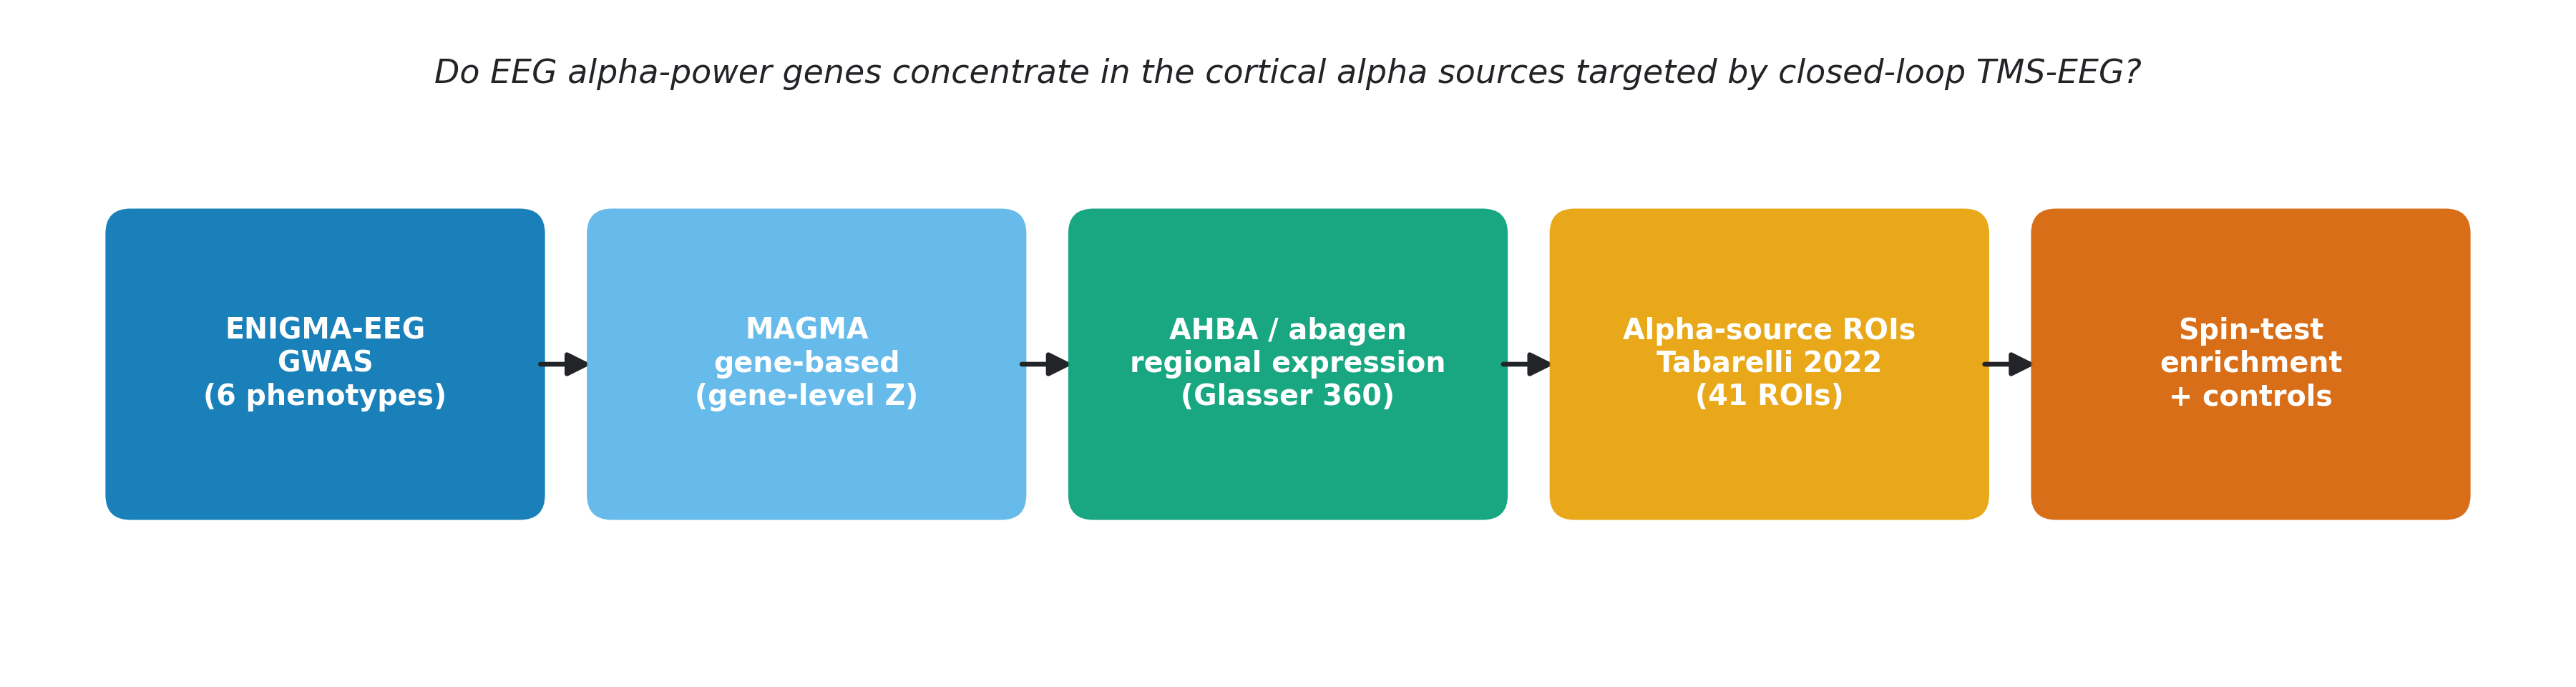
\includegraphics[keepaspectratio,alt={Study design. From the ENIGMA-EEG oscillatory-power GWAS through MAGMA gene-based analysis and AHBA regional expression to the Tabarelli alpha-source ROIs, tested for spatial enrichment against a spin-test null with specificity and robustness controls.}]{figures/fig1_pipeline.png}}
\caption{\textbf{Study design.} From the ENIGMA-EEG oscillatory-power
GWAS through MAGMA gene-based analysis and AHBA regional expression to
the Tabarelli alpha-source ROIs, tested for spatial enrichment against a
spin-test null with specificity and robustness controls.}
\end{figure}

\subsection{2. Methods}\label{methods}

All analyses used publicly available secondary data. No primary data
were collected. Code and derived results are available (see \emph{Data
and code availability}); raw GWAS, AHBA and reference-panel data are
redistributed under their original licences only as download
instructions.

\subsubsection{2.1 GWAS summary
statistics}\label{gwas-summary-statistics}

We obtained ENIGMA-EEG oscillatory-power summary statistics (Smit et
al., 2018; 2018-11-01 release, \texttt{select\_N6000\_Hom100}) for six
scalp-derived phenotypes: alpha power at the central electrode Cz
(\textbf{alphaCz}, the pre-declared primary phenotype), alpha power at
an occipital site (\textbf{alphaOcc}), the occipital alpha peak
frequency (\textbf{peakOcc}, an index of individual alpha frequency),
and --- as specificity controls --- theta, beta and delta power at Cz
(\textbf{thetaCz, betaCz, deltaCz}). Each file contained ≈4.96 million
autosomal SNPs with per-SNP sample size (N ≈ 6,000--7,700). The genome
build was verified as GRCh37/hg19 (e.g., rs3094315 at chr1:752,566),
matching the gene-location and reference-panel builds, so no liftOver
was required.

\subsubsection{2.2 Gene-based analysis
(MAGMA)}\label{gene-based-analysis-magma}

Gene-based association was computed with MAGMA v1.10 (de Leeuw et al.,
2015). SNPs were annotated to genes (build-37 NCBI gene locations;
19,427 genes) with a 35 kb upstream / 10 kb downstream window; the
18,053 genes with ≥1 mapped SNP were carried into the gene-based test.
The SNP-wise mean model used the 1000 Genomes European reference panel
(1000 Genomes Project Consortium, 2015; 503 individuals) to model
linkage disequilibrium. Entrez gene identifiers were mapped to HGNC
symbols using the gene-location file. Gene \emph{p}-values were
corrected by Bonferroni and Benjamini--Hochberg FDR. For the enrichment
analysis we retained (i) the full genome-wide vector of gene-level
\emph{z}-statistics and (ii) a top-100 gene set ranked by gene
\emph{p}-value; threshold-based sets (Bonferroni, FDR,
\emph{p}\textless10⁻³, \emph{p}\textless10⁻²) were also generated for
reference.

\subsubsection{2.3 Regional gene expression (AHBA /
abagen)}\label{regional-gene-expression-ahba-abagen}

Regional transcription was estimated with \emph{abagen} (development
build post-0.1.3, GitHub \texttt{netneurolab/abagen}, required for
pandas ≥2 compatibility; Markello et al., 2021) from AHBA microarray
data (Hawrylycz et al., 2012). Default processing was used
(intensity-based filtering threshold 0.5; probe selection by
differential stability; within-donor scaled robust sigmoid
normalisation; \texttt{missing="interpolate"}; matched-sample
normalisation). Of the six AHBA donors, five were used; donor 15496
(H0351.1015, a left-hemisphere-only donor) was excluded because its
normalized-microarray archive was unavailable at source at the time of
analysis (persistent HTTP 404). The primary parcellation was Glasser
HCP-MMP1.0 (Glasser et al., 2016; 360 regions), matching the space in
which the alpha sources are defined. Because AHBA samples are mapped by
\emph{abagen} to fsaverage5, the Glasser atlas was resampled from
fsLR32k to fsaverage5 using the Human Connectome Project
\texttt{resample\_fsaverage} registration spheres (nearest-neighbour in
the common fsaverage frame); resampling preserved all 180 parcels per
hemisphere. The resulting expression matrix contained 360 regions ×
15,563 genes, with complete coverage of all 82 target parcels. For
robustness, expression was also computed in the Schaefer-100 (Schaefer
et al., 2018) and Yan-600 homotopic (Yan et al., 2023) parcellations,
both in fsaverage5.

\subsubsection{2.4 Alpha-source region
set}\label{alpha-source-region-set}

The 41 alpha-source regions of Tabarelli et al.~(2022) were used as the
target set (16 occipital, 7 parietal, 18 frontal HCP-MMP labels),
applied bilaterally (82 parcels). Because the sources are natively
defined in the Glasser atlas, the mapping is one-to-one by label,
avoiding subjective region translation. A prefrontal-hub subset (areas
8C, 8Av, 9a; 6 parcels) was additionally tested, motivated by the
paper's identification of 8C as the principal connectivity hub. For the
Schaefer-100 and Yan-600 sensitivity analyses, the alpha-source set was
re-mapped by fsaverage5 surface overlap: a parcel was flagged as target
if ≥50\% of its cortical vertices fell within the Glasser alpha-source
set (31/100 Schaefer parcels; 180/600 Yan parcels).

\begin{figure}
\centering
\pandocbounded{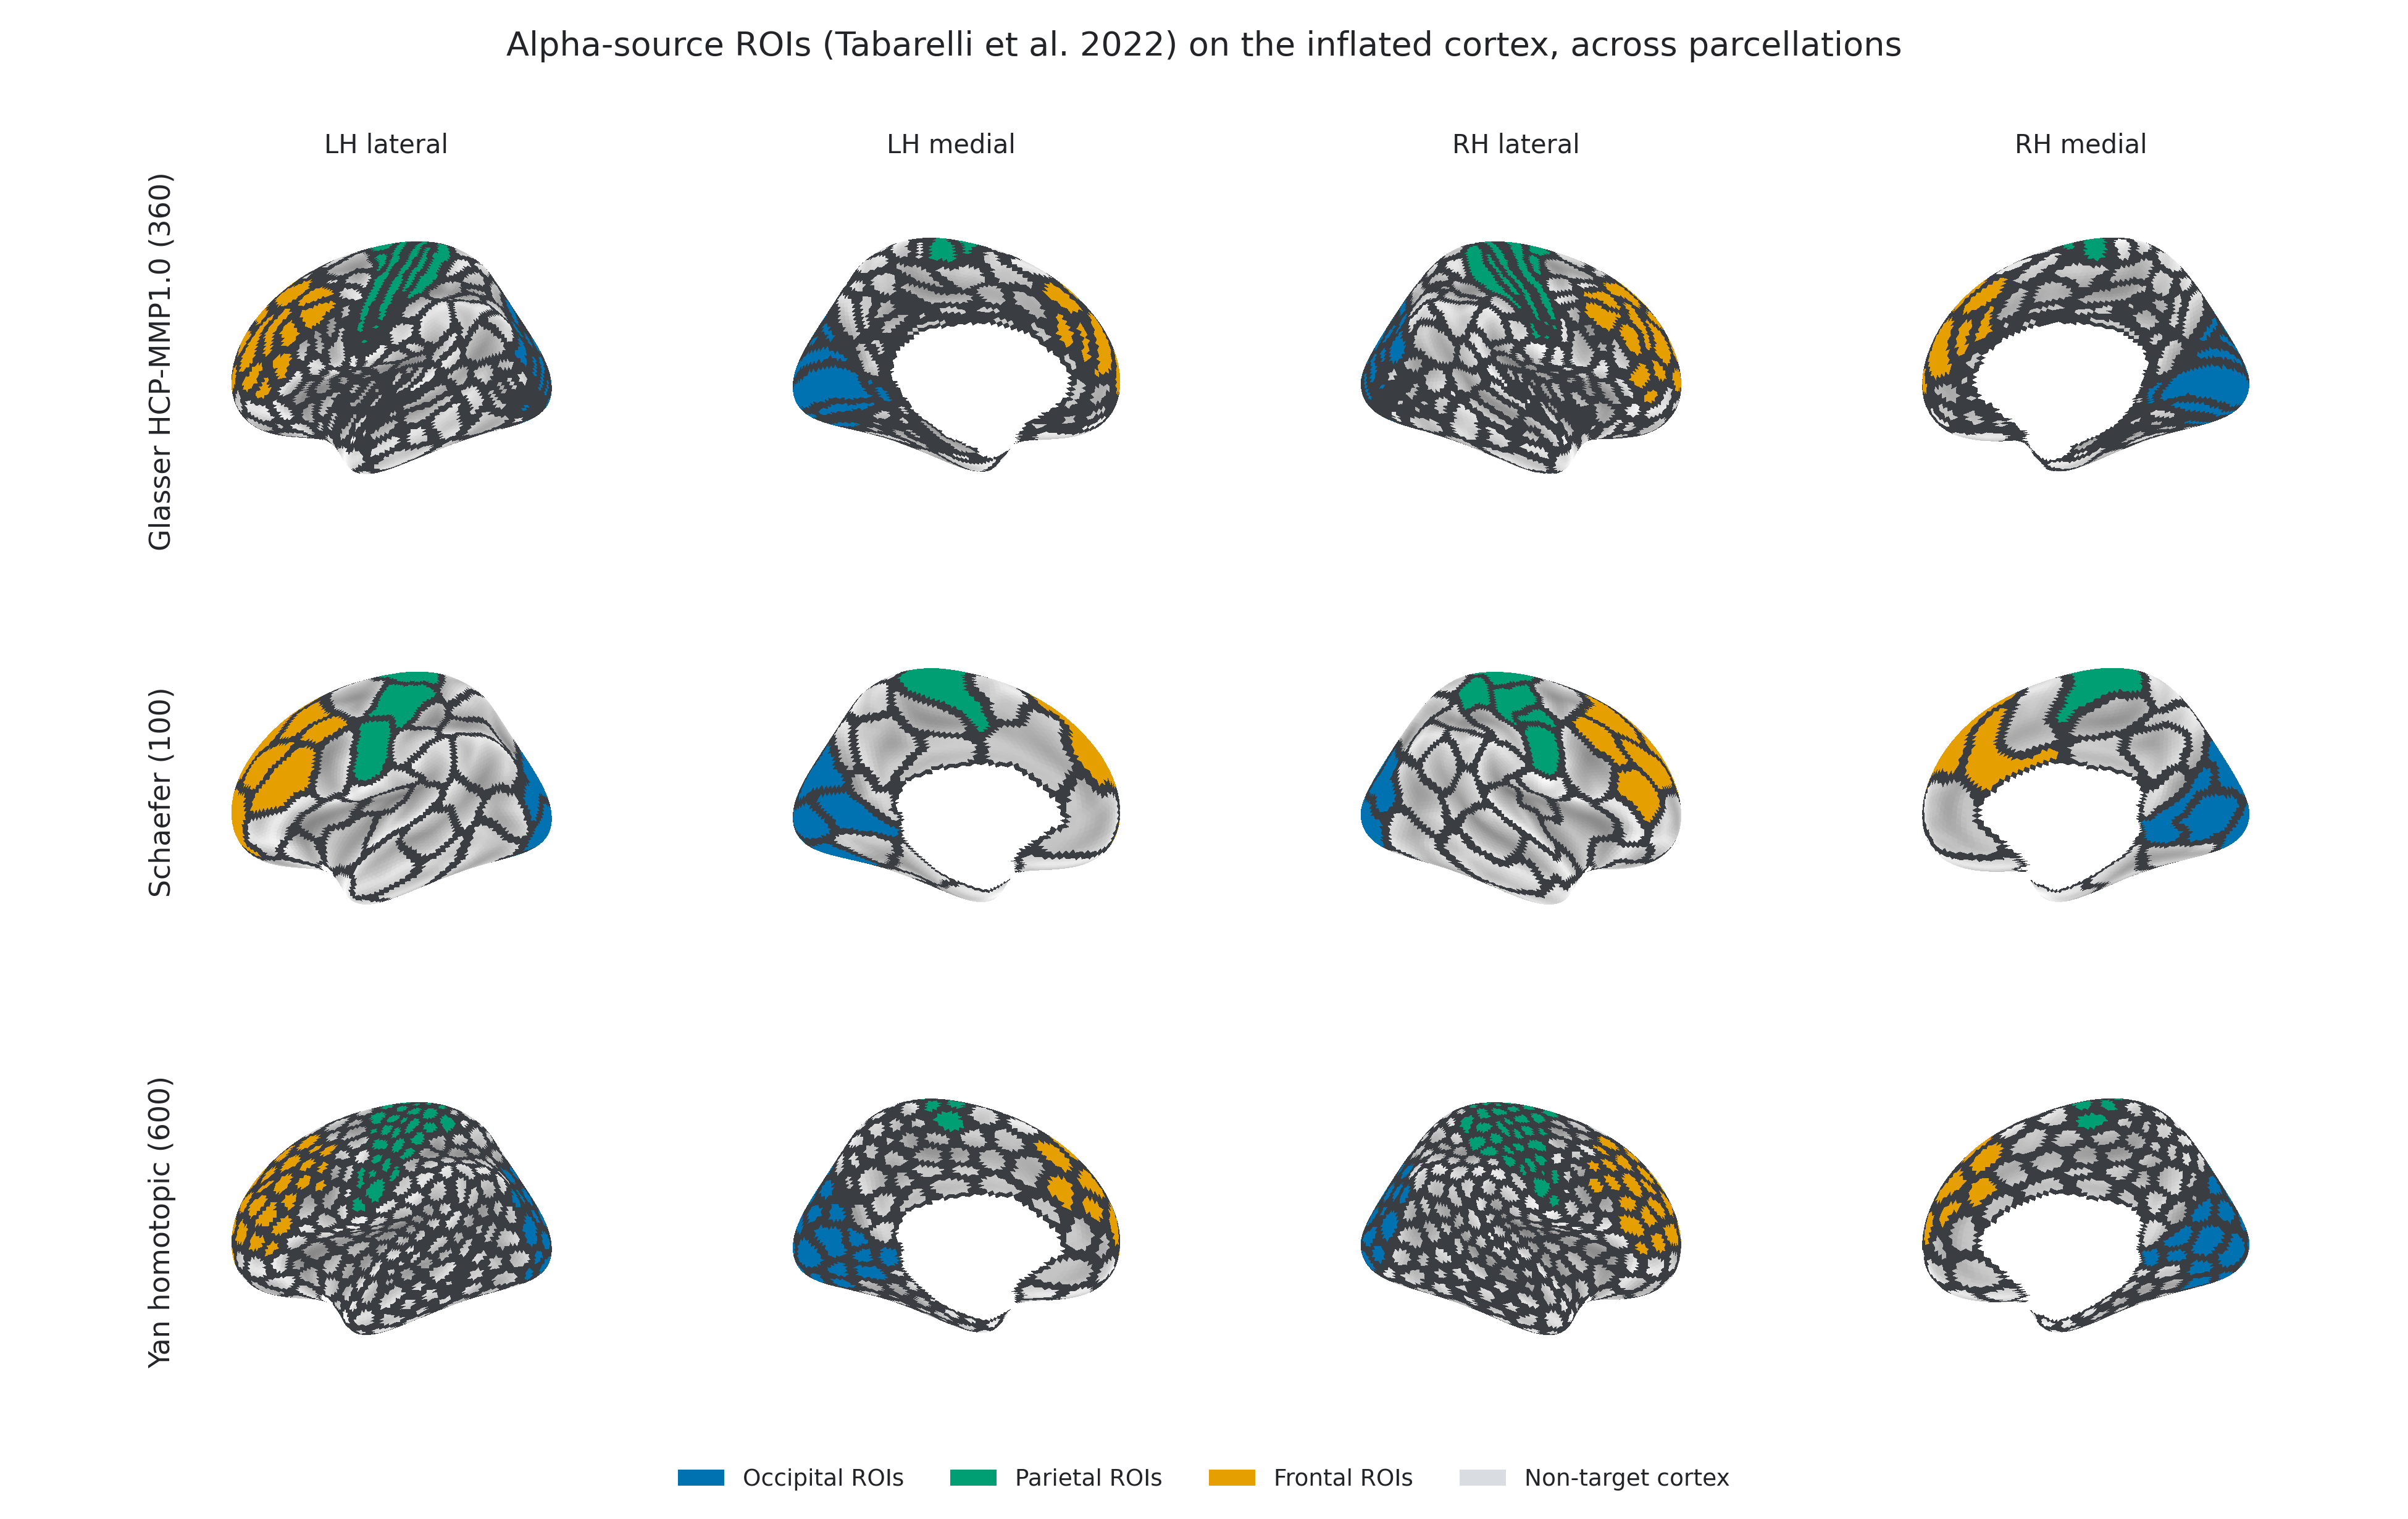
\includegraphics[keepaspectratio,alt={Alpha-source ROIs on the inflated cortex, across parcellations. The 41 Tabarelli alpha-source regions (bilateral) shown on the fsaverage5 inflated surface for Glasser HCP-MMP1.0, Schaefer-100 and Yan-600. In every parcellation the target parcels are coloured by sector (occipital, parietal, frontal); for Schaefer and Yan each target parcel takes the sector of the Glasser alpha-source it most overlaps. Thin dark lines are atlas parcel boundaries; grey is non-target cortex.}]{figures/fig2_atlas_rois.png}}
\caption{\textbf{Alpha-source ROIs on the inflated cortex, across
parcellations.} The 41 Tabarelli alpha-source regions (bilateral) shown
on the fsaverage5 inflated surface for Glasser HCP-MMP1.0, Schaefer-100
and Yan-600. In every parcellation the target parcels are coloured by
sector (occipital, parietal, frontal); for Schaefer and Yan each target
parcel takes the sector of the Glasser alpha-source it most overlaps.
Thin dark lines are atlas parcel boundaries; grey is non-target cortex.}
\end{figure}

\subsubsection{2.5 Alpha transcriptomic score and enrichment
test}\label{alpha-transcriptomic-score-and-enrichment-test}

We defined two per-region scores. The \textbf{continuous} score is the
Spearman correlation, across all genes shared between the expression
matrix and the gene-based results, between a region's expression profile
and the genome-wide gene-level \emph{z}-statistics; it uses the full
association signal without any significance threshold. The
\textbf{top-100} score is the mean \emph{z}-scored expression, across
regions, of the top-100 gene set. Enrichment was quantified as the
difference between the mean score in the target regions and the rest of
cortex.

Statistical significance was assessed against a spin-test null that
preserves the spatial autocorrelation of cortical maps (Alexander-Bloch
et al., 2018). Because the parcellation was surface-based, we generated
10,000 spatial rotations of the parcel centroids on the fsaverage5
sphere (nearest-neighbour reassignment; left- and right-hemisphere
rotations mirror-matched; seed fixed and logged), and computed a
one-sided \emph{p}-value (H1: target \textgreater{} rest) as the
fraction of rotated maps with a target-region mean at least as large as
observed. This self-contained implementation was used because the spin
generator had been removed from the version of \emph{netneurotools}
available at analysis time. Specificity and replication were assessed by
repeating the test for all six phenotypes and both scores, and
correcting the resulting 24-cell grid by Benjamini--Hochberg FDR.
Robustness was assessed by repeating the primary-phenotype test in the
Schaefer-100 and Yan-600 parcellations. Because the analysis is
internally power-matched --- every phenotype shares the same GWAS
design, the same expression matrix and the same null --- the
\emph{relative} comparison between the alpha and control bands is
informative about specificity independent of the absolute statistical
power of any single GWAS.

\subsubsection{2.6 Validation and complementary
nulls}\label{validation-and-complementary-nulls}

Three analyses established the validity of the enrichment test.
\textbf{(i) Positive control.} To confirm that the pipeline can detect a
genuine spatial effect, we replaced the gene statistic with the gene
loadings of the first principal component (PC1) of the AHBA expression
matrix --- the dominant, well-replicated cortical expression gradient
--- and set the target to the top-tertile PC1 regions; a correct
pipeline must recover a highly significant enrichment. \textbf{(ii)
Co-expression-aware gene-set null.} Because gene-set enrichment on AHBA
is prone to false positives from within-set spatial co-expression
(Fulcher et al., 2021), we complemented the spin test (which permutes
space) with a gene-set null for the top-100 analysis: 10,000 random gene
sets of matched size were drawn, and \emph{p}\_geneset was the fraction
whose target-versus-rest difference met or exceeded the observed value.
\textbf{(iii) Spin validation.} Because the spin generator was
self-implemented, we benchmarked it against an independent
spatial-autocorrelation-preserving surrogate model (brainsmash; Burt et
al., 2020; Markello \& Misić, 2021), generating 1,000 surrogate maps of
the primary alpha score over a Euclidean parcel-distance matrix and
comparing the resulting \emph{p}-value with the spin \emph{p}-value.

\subsubsection{2.7 Reproducibility}\label{reproducibility}

Every stage logged its parameters (random seed, parcellation version,
\emph{abagen} and package versions, MAGMA build) to a machine-readable
run log. A global seed (20260721) governed all permutations. Analyses
ran under Python 3.12.

\subsection{3. Results}\label{results}

\subsubsection{3.1 Gene-based analysis recovers credible
signal}\label{gene-based-analysis-recovers-credible-signal}

MAGMA gene-based analysis of central alpha power tested 18,053 genes. A
single gene survived genome-wide Bonferroni and FDR correction ---
\emph{PRKG2} (\emph{p} = 4.0 × 10⁻⁷, \emph{q} = 0.007) --- consistent
with the modest sample size. The leading sub-threshold signal included
the chr3p21 pleiotropic cluster (\emph{GNL3}, \emph{GLT8D1},
\emph{NT5DC2}, \emph{PBRM1}; \emph{p} ≈ 4--5 × 10⁻⁵), one of the most
robust loci in psychiatric genetics and consistent with the ENIGMA-EEG
thesis that psychiatric-liability genes contribute to oscillatory brain
activity (Smit et al., 2018). The presence of this expected locus
provides a positive control that the gene-based pipeline behaves
correctly. Because only one gene survived strict correction, we did not
treat a threshold-based gene set as the primary readout; instead the
continuous score (using the full gene-level signal) was pre-declared
primary and the top-100 gene set served as a sensitivity analysis. (The
analysis grid was fixed in advance but was not formally pre-registered.)

\begin{figure}
\centering
\pandocbounded{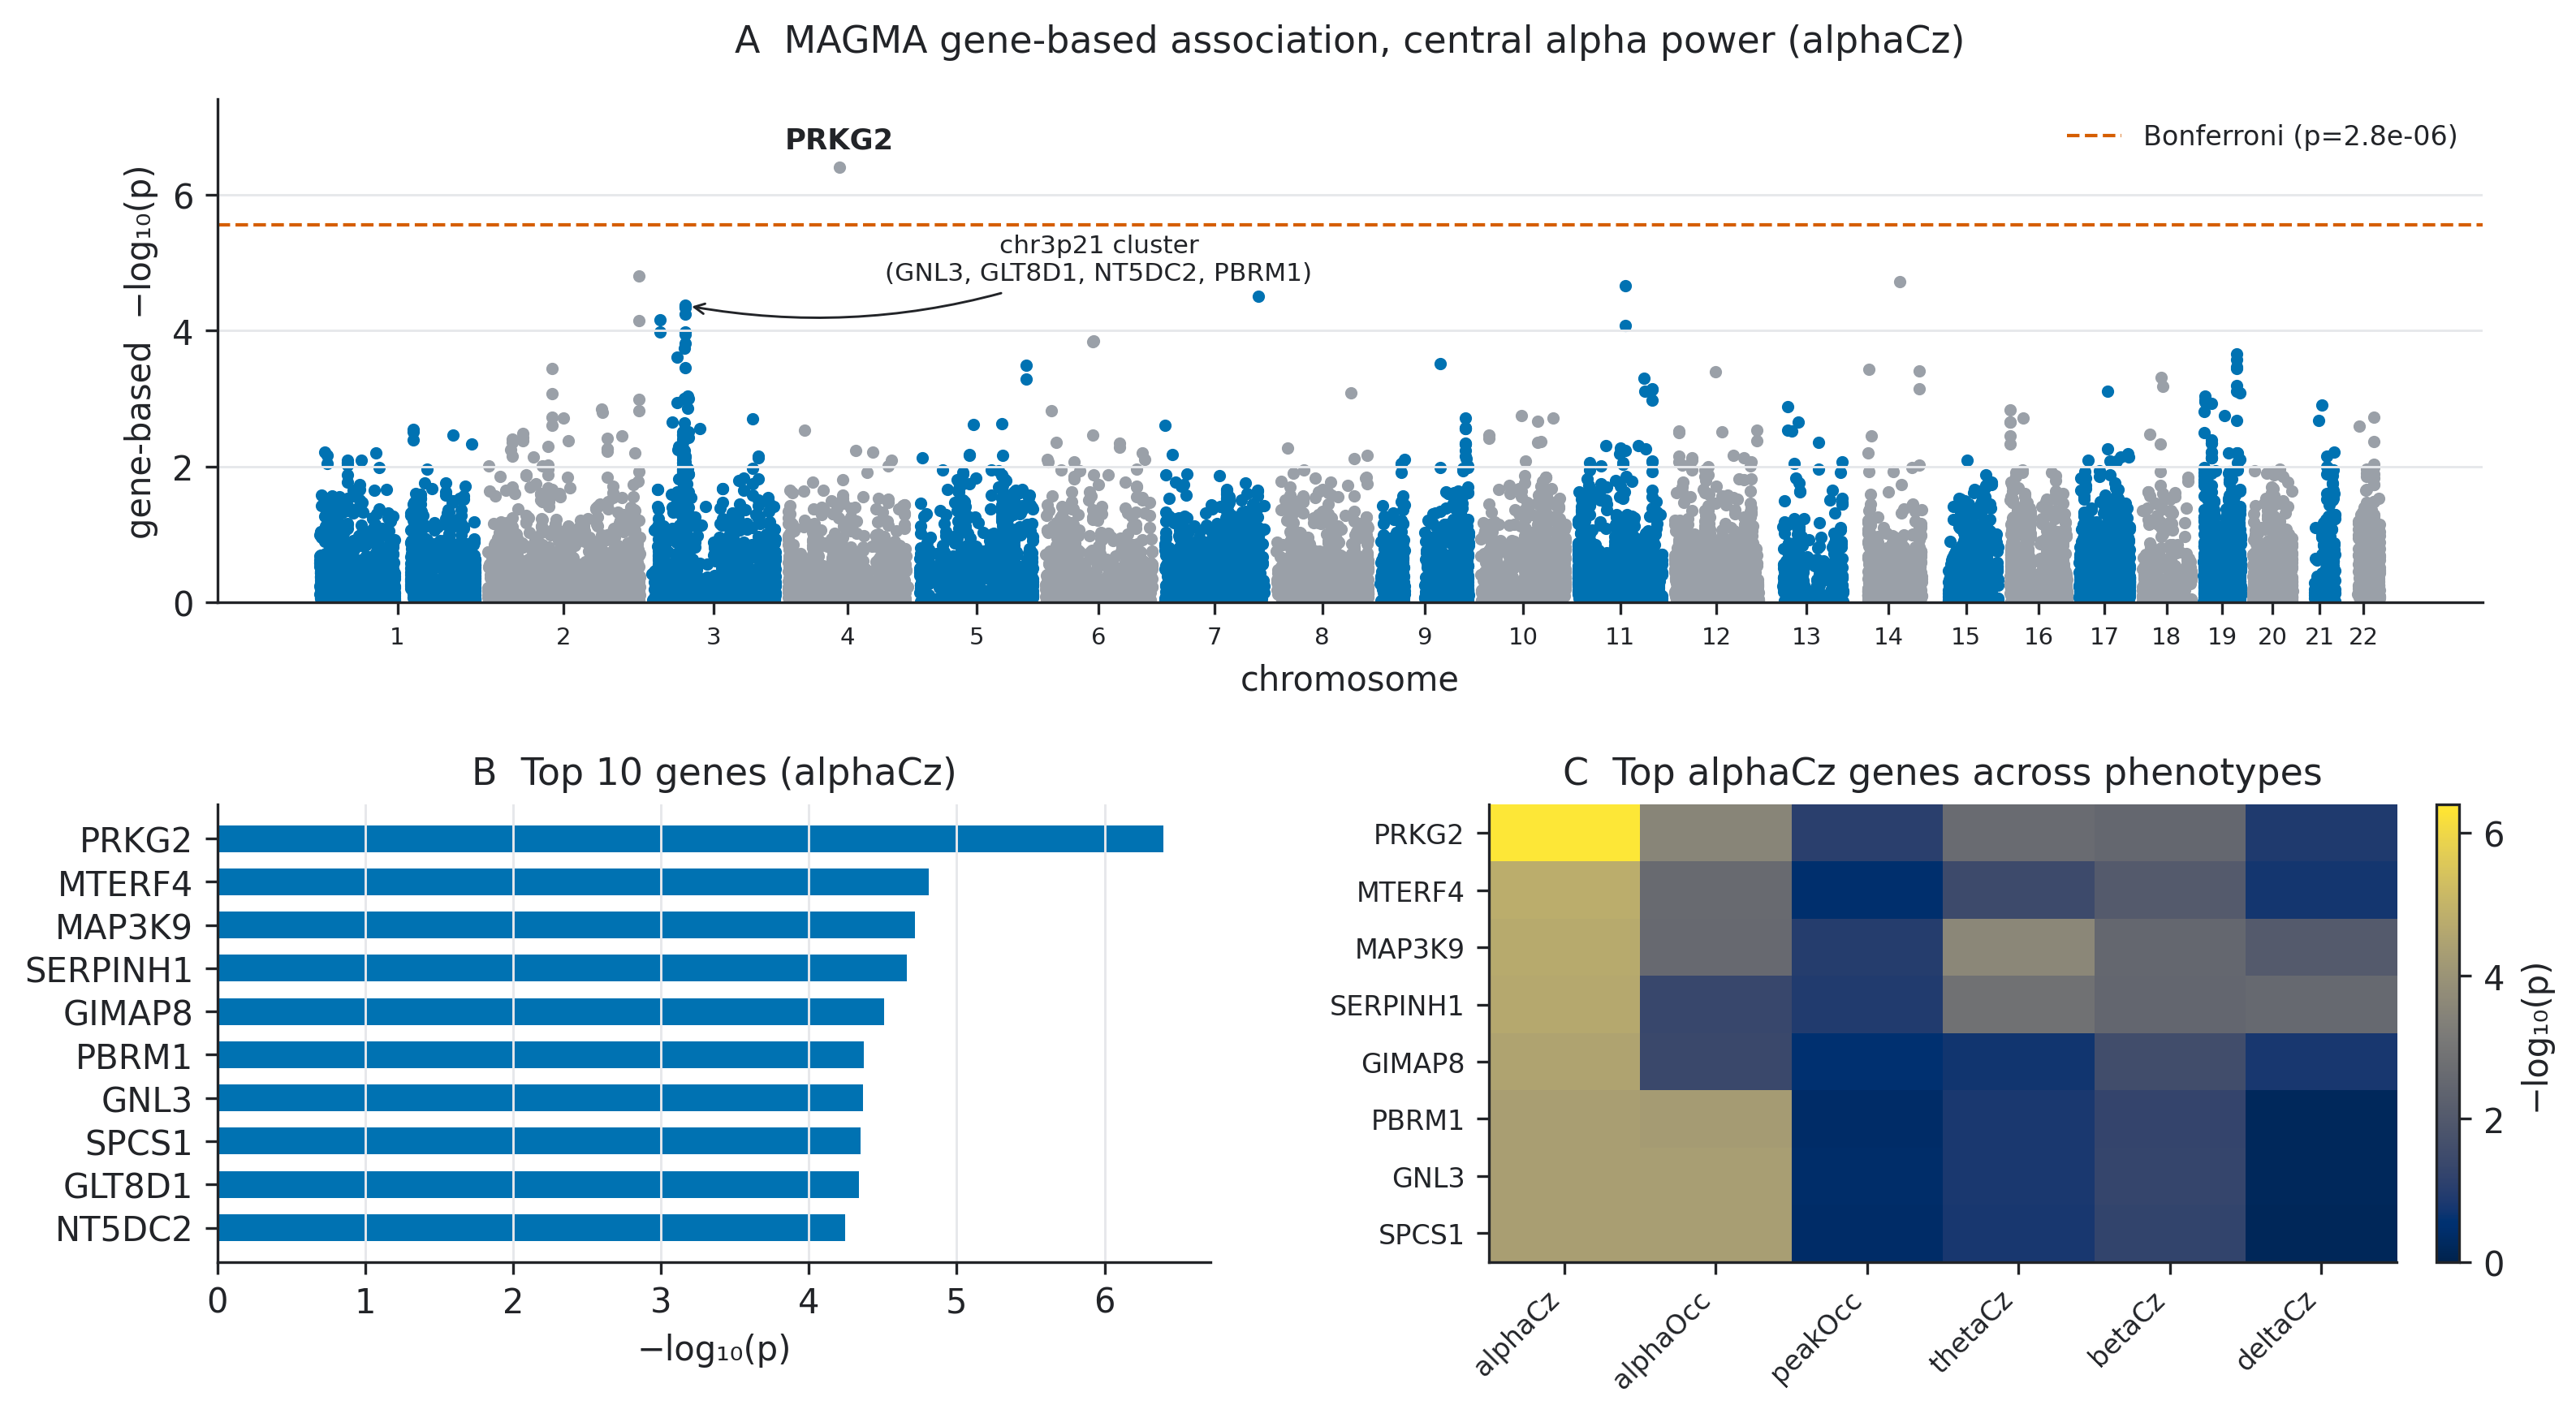
\includegraphics[keepaspectratio,alt={Gene-based genetics. (A) MAGMA gene-based association for central alpha power (alphaCz); PRKG2 passes Bonferroni and the chr3p21 pleiotropic cluster is the leading sub-threshold signal. (B) Top-10 genes. (C) −log₁₀ p of the top alphaCz genes across all six phenotypes --- the gene-level signal is largely specific to alphaCz.}]{figures/fig3_genetics.png}}
\caption{\textbf{Gene-based genetics.} (A) MAGMA gene-based association
for central alpha power (alphaCz); \emph{PRKG2} passes Bonferroni and
the chr3p21 pleiotropic cluster is the leading sub-threshold signal. (B)
Top-10 genes. (C) −log₁₀ \emph{p} of the top alphaCz genes across all
six phenotypes --- the gene-level signal is largely specific to
alphaCz.}
\end{figure}

\subsubsection{3.2 The enrichment test is valid and the custom spin is
corroborated}\label{the-enrichment-test-is-valid-and-the-custom-spin-is-corroborated}

The positive control confirmed that the pipeline detects genuine spatial
structure: with the PC1 expression-gradient loadings as the gene
statistic and the top-tertile PC1 regions as the target, the spin test
recovered a large, highly significant enrichment (target-versus-rest
difference = 0.74; \emph{p}\_spin = 2 × 10⁻⁴). The subsequent alpha
nulls are therefore not a floor effect of an insensitive method. The
self-implemented spin was corroborated by an independent surrogate
model: for the primary alpha map, the spin \emph{p}-value (0.022) and
the brainsmash \emph{p}-value (0.018) were closely concordant.

\begin{figure}
\centering
\pandocbounded{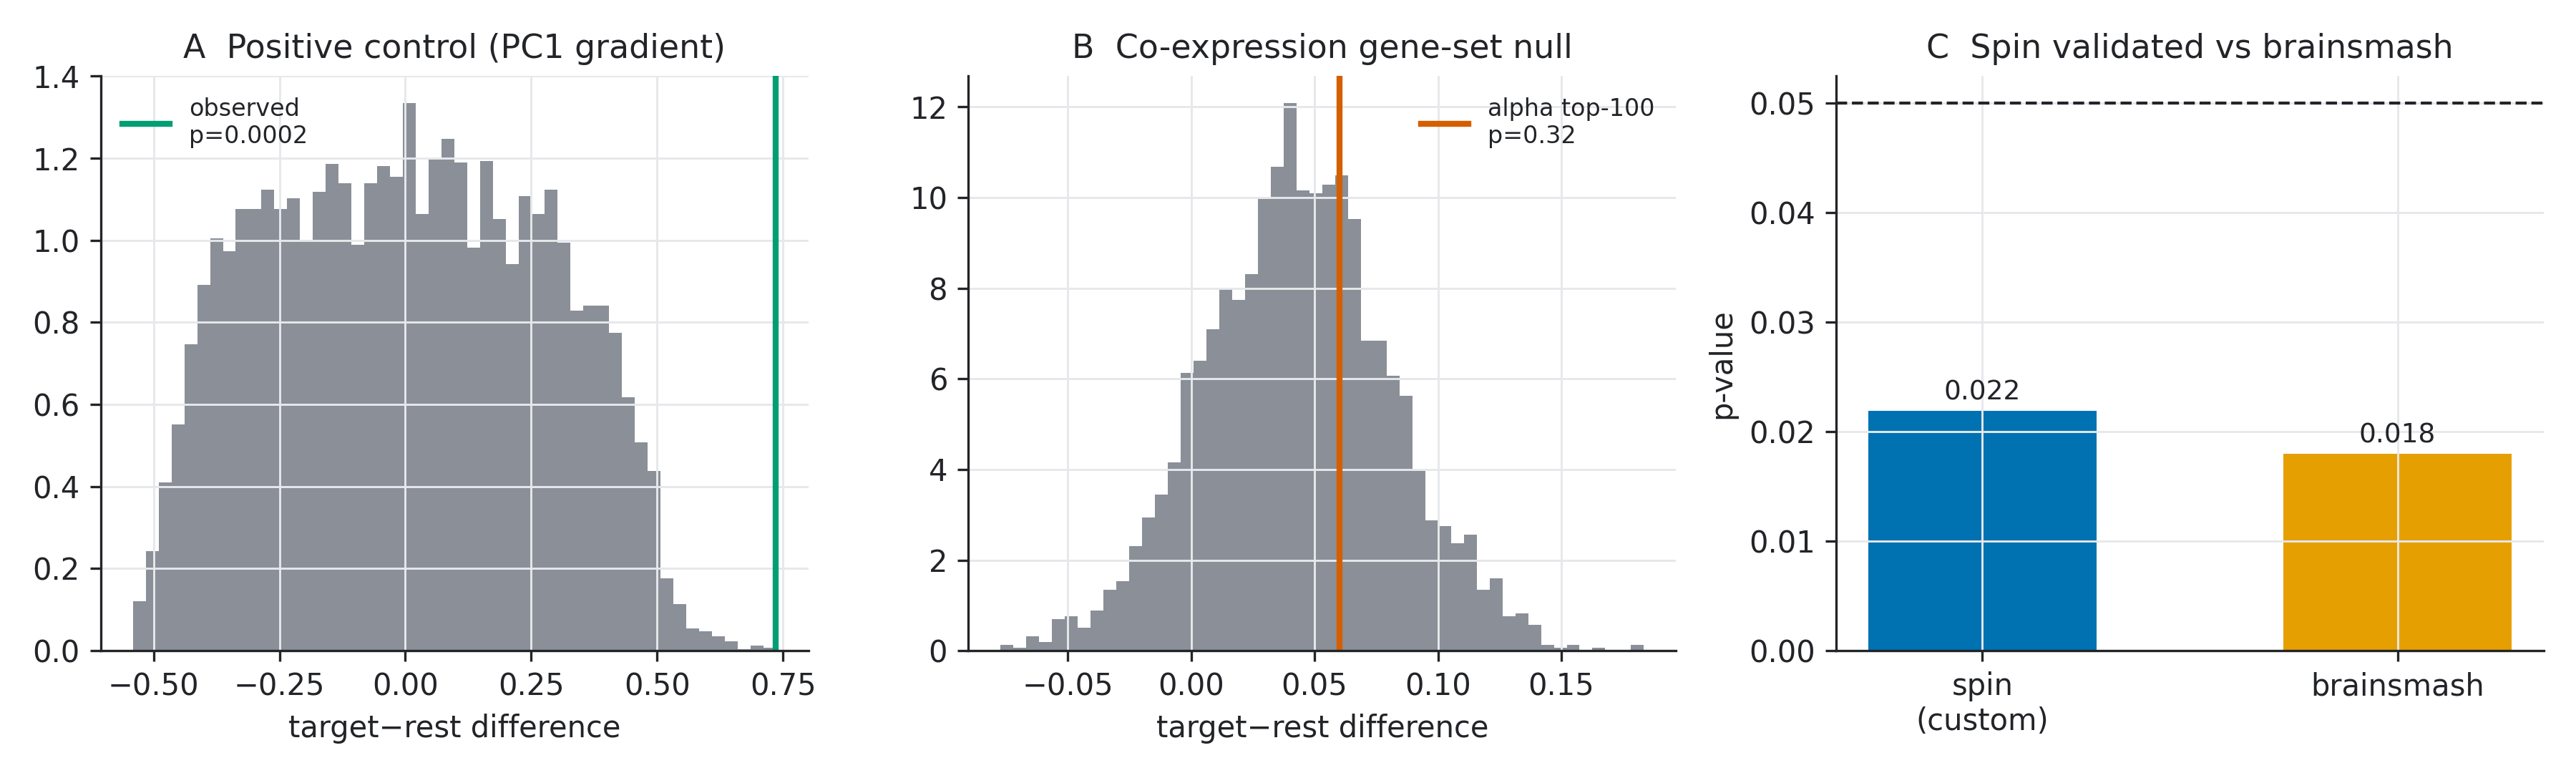
\includegraphics[keepaspectratio,alt={Validation of the enrichment test. (A) Positive control: with the dominant expression gradient (PC1) as the gene statistic, the spin test recovers a large enrichment (p\_spin = 2 × 10⁻⁴). (B) Co-expression-aware gene-set null: the alpha top-100 target-versus-rest difference sits at the centre of 10,000 random gene sets (p\_geneset = 0.33). (C) The custom spin agrees with brainsmash surrogates.}]{figures/fig6_validation.png}}
\caption{\textbf{Validation of the enrichment test.} (A) Positive
control: with the dominant expression gradient (PC1) as the gene
statistic, the spin test recovers a large enrichment (\emph{p}\_spin = 2
× 10⁻⁴). (B) Co-expression-aware gene-set null: the alpha top-100
target-versus-rest difference sits at the centre of 10,000 random gene
sets (\emph{p}\_geneset = 0.33). (C) The custom spin agrees with
brainsmash surrogates.}
\end{figure}

\subsubsection{3.3 Primary phenotype: nominal but modest
enrichment}\label{primary-phenotype-nominal-but-modest-enrichment}

In the primary Glasser parcellation, central alpha power showed nominal
enrichment of alpha transcriptomic signal in the 41 alpha-source regions
for both scores: the continuous score gave a target-versus-rest
difference corresponding to \emph{z} = 1.98 relative to the spin null
(\emph{p}\_spin = 0.022), and the top-100 score gave \emph{z} = 1.77
(\emph{p}\_spin = 0.030). The prefrontal-hub subset (8C, 8Av, 9a) was
not significant for either score (continuous \emph{p}\_spin = 0.11;
top-100 \emph{p}\_spin = 0.73), indicating that any enrichment was
distributed across the broad alpha-source network rather than
concentrated at the connectivity hubs. Taken alone, this primary result
is compatible with H1.

\begin{figure}
\centering
\pandocbounded{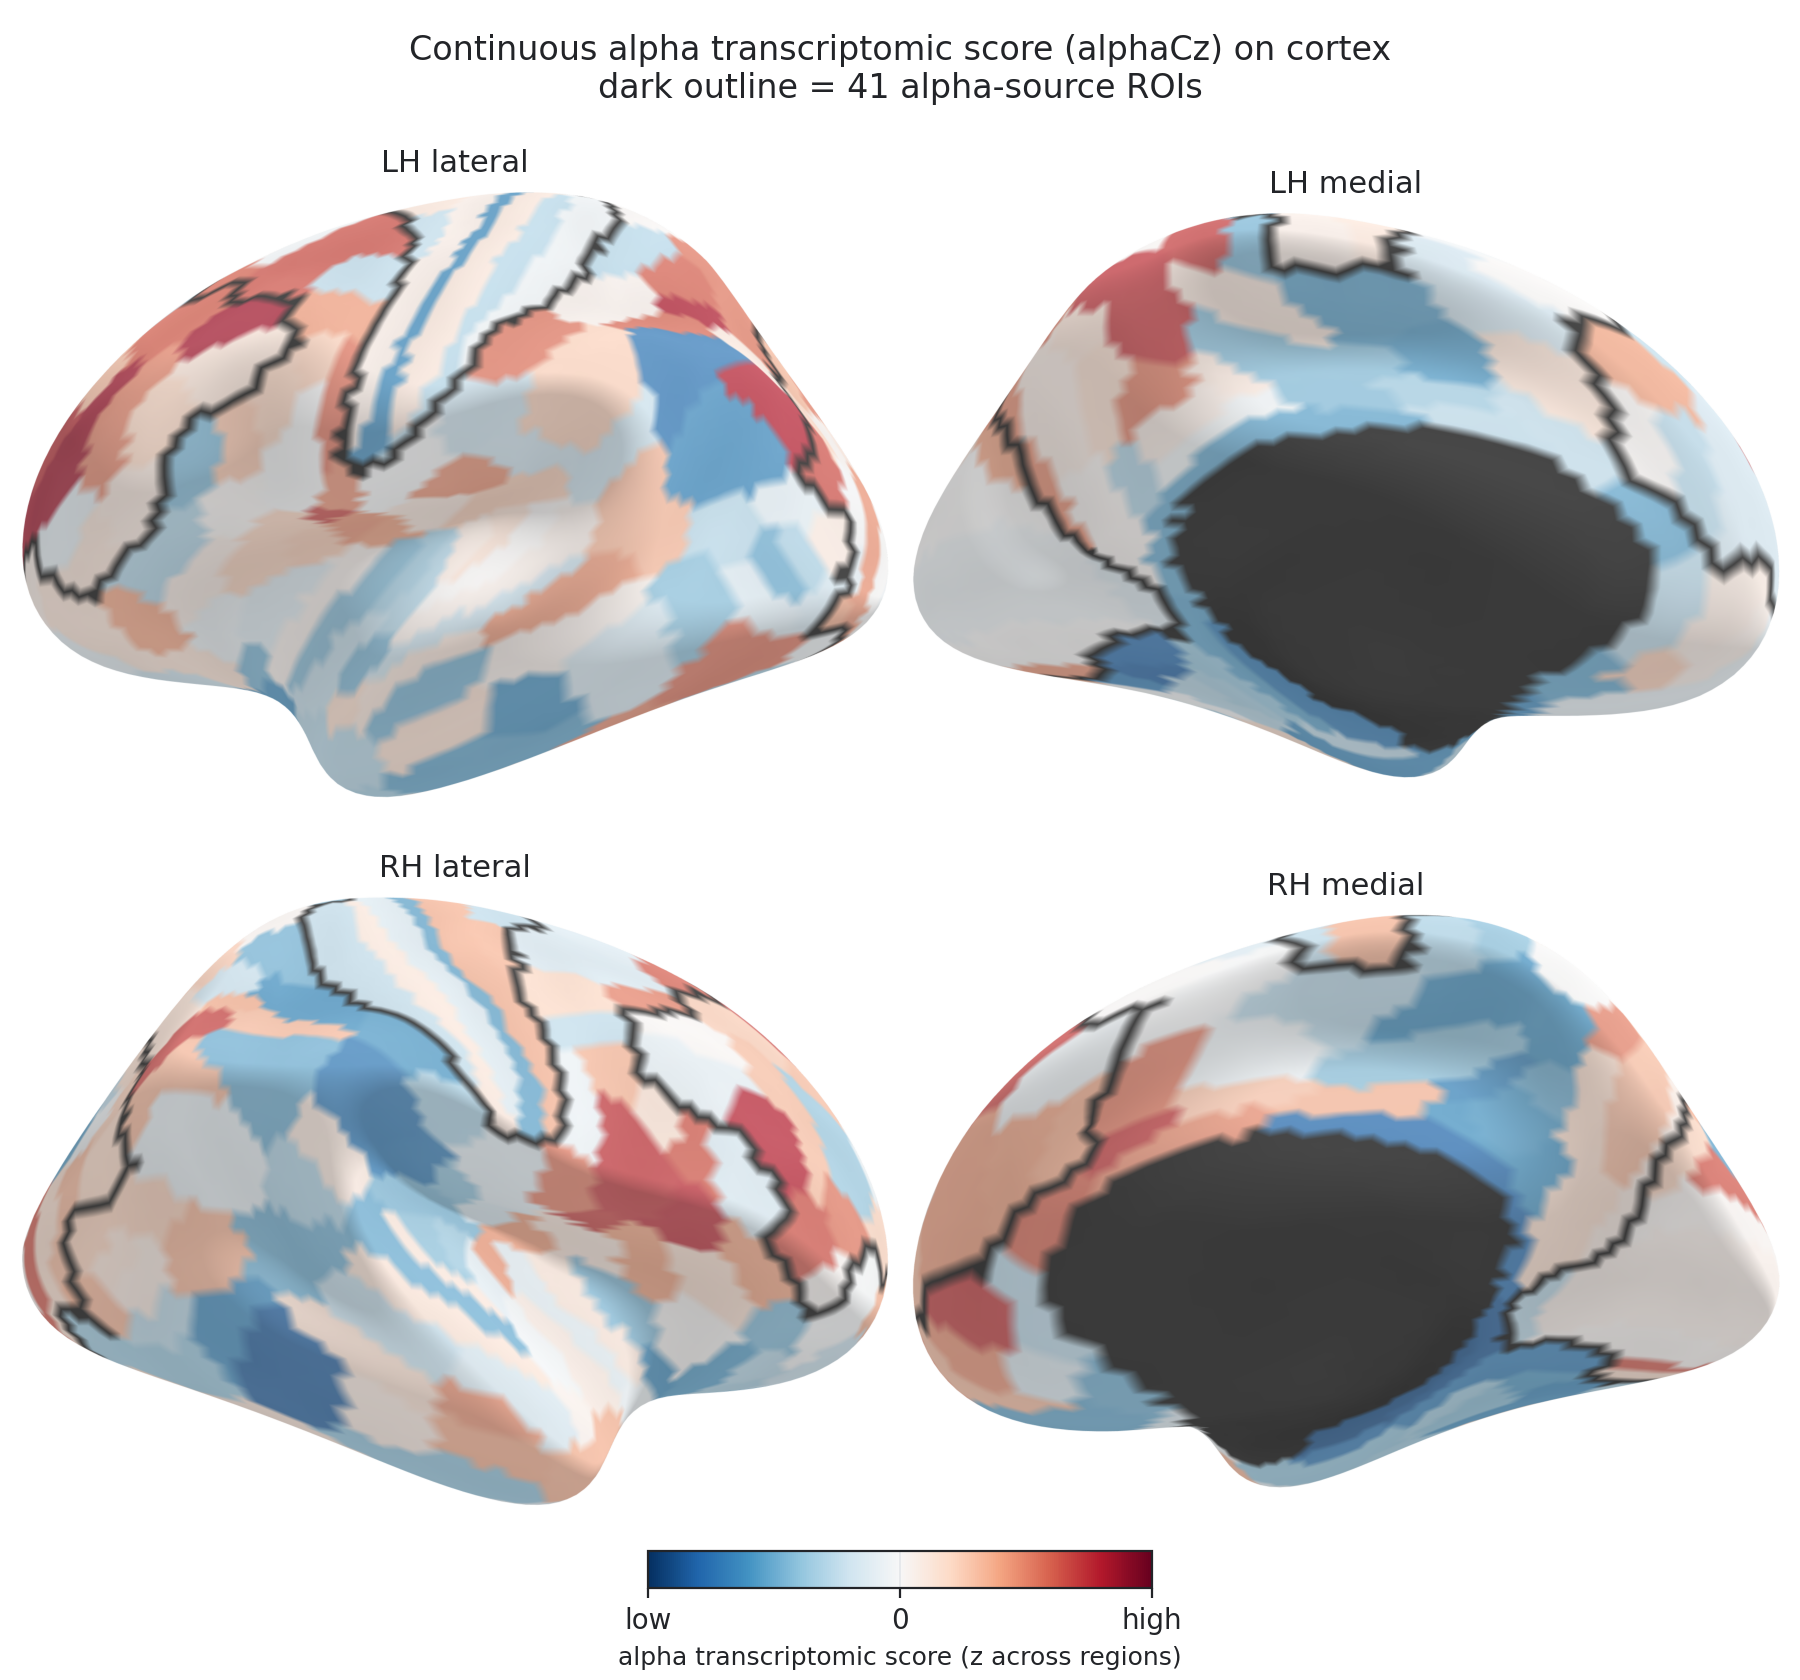
\includegraphics[keepaspectratio,alt={Alpha transcriptomic score on the cortex. The continuous alpha score (alphaCz) per Glasser region, tertile-binned for display, on the inflated surface; the black outline marks the 41 alpha-source ROIs. The score is weakly and diffusely patterned and is not concentrated within the target ROIs.}]{figures/fig4_score_map.png}}
\caption{\textbf{Alpha transcriptomic score on the cortex.} The
continuous alpha score (alphaCz) per Glasser region, tertile-binned for
display, on the inflated surface; the black outline marks the 41
alpha-source ROIs. The score is weakly and diffusely patterned and is
not concentrated within the target ROIs.}
\end{figure}

\subsubsection{3.4 Specificity and replication: the effect is not
alpha-specific}\label{specificity-and-replication-the-effect-is-not-alpha-specific}

Repeating the test across all six phenotypes overturned the primary
interpretation (Table 1). In the continuous score, the theta control
band was also nominally enriched in the alpha-source regions
(\emph{p}\_spin = 0.042), while the occipital alpha phenotype --- the
natural replication of the central alpha result --- was not
(\emph{p}\_spin = 0.20). In the top-100 score, the pattern was still
less specific: the occipital alpha phenotype (\emph{p}\_spin = 0.008)
and the beta control band (\emph{p}\_spin = 0.011) gave the strongest
signals of all, both exceeding central alpha (\emph{p}\_spin = 0.030),
with delta also nominally significant (\emph{p}\_spin = 0.042). The
alpha peak-frequency (IAF) phenotype --- arguably the most
closed-loop-relevant, since the controller locks to it --- was not
significant for either score (continuous \emph{p}\_spin = 0.13; top-100
\emph{p}\_spin = 0.066). Critically, after Benjamini--Hochberg
correction across the 24-cell phenotype × score × region-set grid,
\textbf{no test remained significant} (minimum \emph{q} = 0.127). The
prefrontal-hub subset was null or negative throughout.

The co-expression-aware gene-set null reinforced this conclusion. When
the alpha top-100 enrichment was tested not against a spatial null but
against 10,000 random gene sets of the same size, the observed
target-versus-rest difference (0.060) was unremarkable --- it fell near
the centre of the random-gene-set distribution (mean 0.043;
\emph{p}\_geneset = 0.33). In other words, the nominal spin-test
enrichment of the alpha gene set reflects a generic tendency of
arbitrary gene sets to be marginally over-expressed in this
occipito-parieto-frontal territory, rather than anything specific to
alpha-associated genes --- precisely the co-expression-driven inflation
that spatial-only nulls do not capture (Fulcher et al., 2021).

\textbf{Table 1.} Spin-test enrichment of alpha transcriptomic signal in
the 41 alpha-source regions (Glasser HCP-MMP1.0), by phenotype and
score. \emph{z} is relative to the 10,000-rotation spin null;
\emph{p}\_spin is one-sided (target \textgreater{} rest); \emph{q} is
Benjamini--Hochberg FDR across the full 24-cell (6 phenotype × 2 score ×
2 region-set) grid. Band labels distinguish alpha power, the alpha
peak-frequency (IAF) phenotype, and the non-alpha control bands.

{\def\LTcaptype{none} % do not increment counter
\begin{longtable}[]{@{}llllll@{}}
\toprule\noalign{}
Score & Phenotype & Band & \emph{z} vs null & \emph{p}\_spin & \emph{q}
(FDR) \\
\midrule\noalign{}
\endhead
\bottomrule\noalign{}
\endlastfoot
Continuous & alphaCz & alpha-power & 1.98 & 0.022 & 0.169 \\
Continuous & alphaOcc & alpha-power & 0.87 & 0.203 & 0.325 \\
Continuous & peakOcc & alpha-frequency & 1.16 & 0.130 & 0.283 \\
Continuous & thetaCz & control & 1.68 & 0.042 & 0.169 \\
Continuous & betaCz & control & 1.22 & 0.123 & 0.283 \\
Continuous & deltaCz & control & 0.99 & 0.168 & 0.310 \\
Top-100 & alphaCz & alpha-power & 1.77 & 0.030 & 0.169 \\
Top-100 & alphaOcc & alpha-power & 2.28 & 0.008 & 0.127 \\
Top-100 & peakOcc & alpha-frequency & 1.72 & 0.066 & 0.227 \\
Top-100 & betaCz & control & 2.13 & 0.011 & 0.127 \\
Top-100 & deltaCz & control & 1.62 & 0.042 & 0.169 \\
Top-100 & thetaCz & control & 1.32 & 0.079 & 0.237 \\
\end{longtable}
}

\subsubsection{3.5 Parcellation sensitivity: direction consistent,
significance
fragile}\label{parcellation-sensitivity-direction-consistent-significance-fragile}

For the primary phenotype, the direction of the continuous-score
enrichment was consistent across all three parcellations (positive;
\emph{z} between 1.5 and 2.0), but nominal significance was reached only
in the native Glasser space (Table 2). Coarsening the parcellation to
Schaefer-100 --- which more closely matches the spatial resolution of
MEG source reconstruction --- did \textbf{not} strengthen the effect
(\emph{p}\_spin = 0.071); refining it to Yan-600 gave a similar trend
(\emph{p}\_spin = 0.058). The top-100 score was significant only in the
Glasser parcellation. Thus the enrichment does not survive a change of
parcellation, and the resolution-matching prediction --- that a coarser
atlas would recover a signal blurred at fine resolution --- was not
borne out.

\begin{figure}
\centering
\pandocbounded{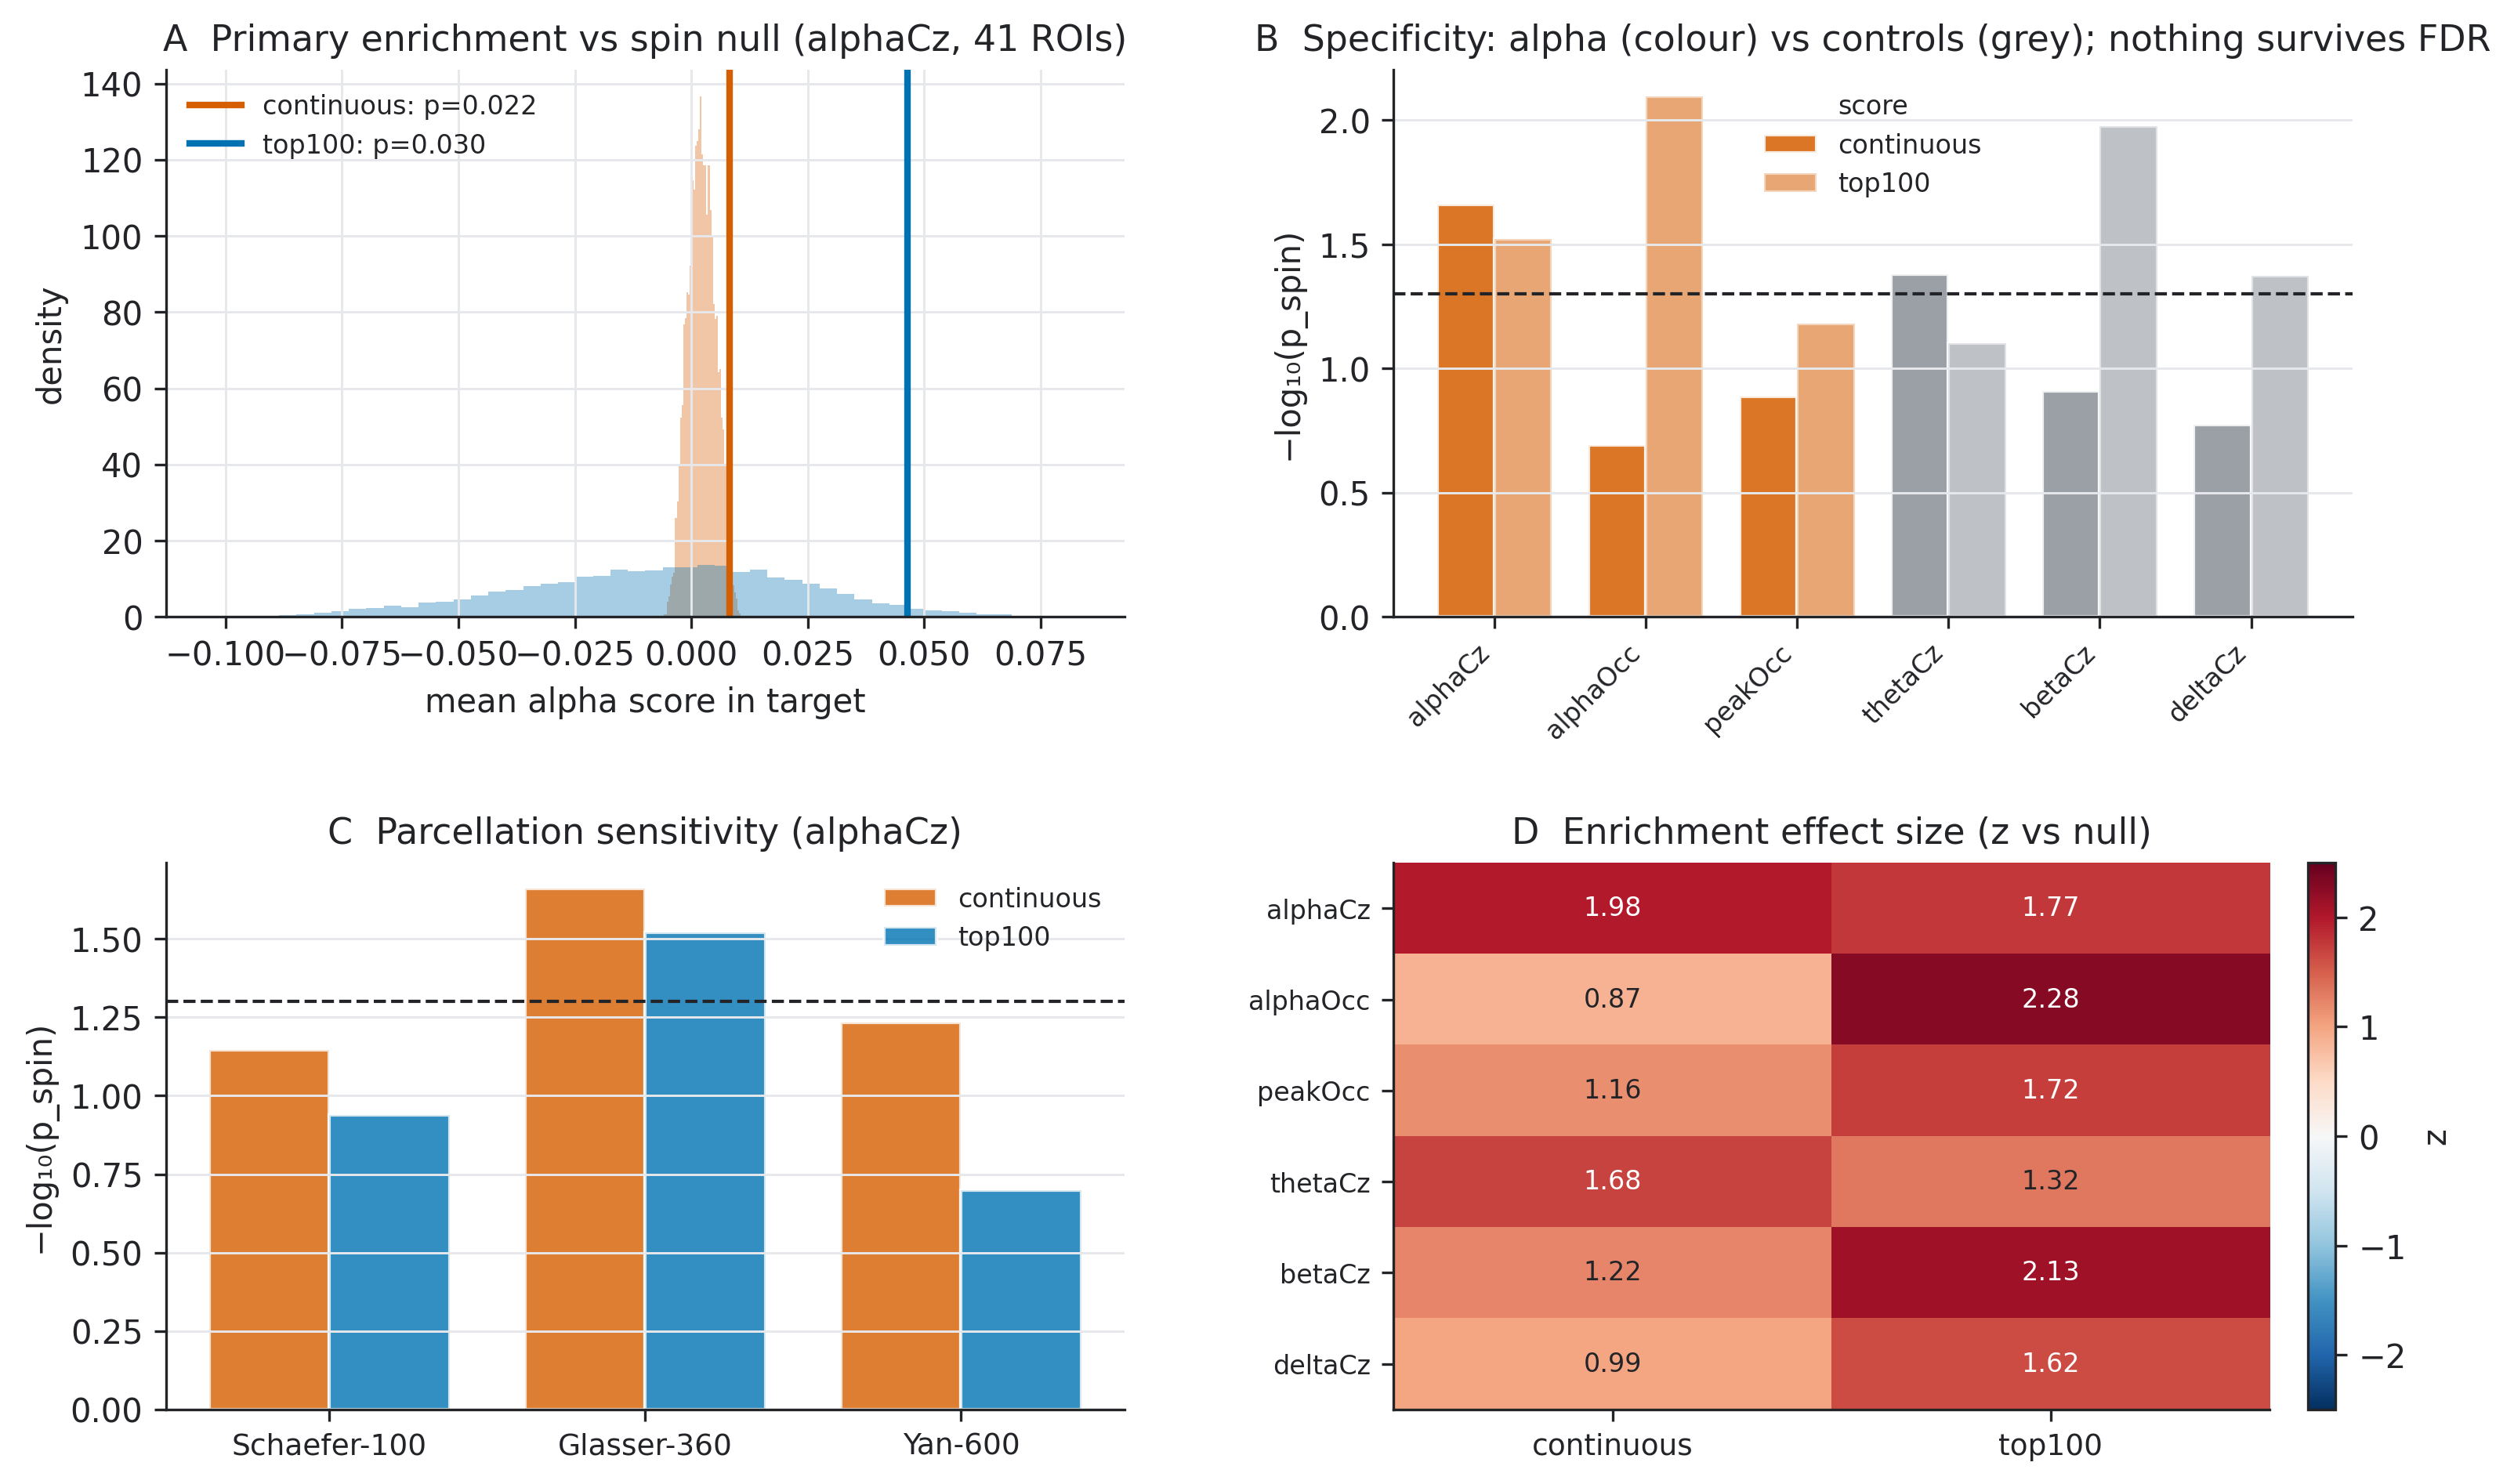
\includegraphics[keepaspectratio,alt={Enrichment, specificity and robustness. (A) Primary alphaCz enrichment against the spin null (both scores). (B) Specificity across the six phenotypes (alpha in colour, controls in grey; dashed line p = 0.05); control bands enrich comparably or more, and nothing survives FDR. (C) Parcellation sensitivity: nominal significance only in the native Glasser space. (D) Enrichment effect size (z vs null) across phenotypes and scores.}]{figures/fig5_enrichment.png}}
\caption{\textbf{Enrichment, specificity and robustness.} (A) Primary
alphaCz enrichment against the spin null (both scores). (B) Specificity
across the six phenotypes (alpha in colour, controls in grey; dashed
line \emph{p} = 0.05); control bands enrich comparably or more, and
nothing survives FDR. (C) Parcellation sensitivity: nominal significance
only in the native Glasser space. (D) Enrichment effect size (\emph{z}
vs null) across phenotypes and scores.}
\end{figure}

\textbf{Table 2.} Parcellation sensitivity for central alpha power
(alphaCz). Target counts reflect the fraction of parcels overlapping the
Glasser alpha-source set.

{\def\LTcaptype{none} % do not increment counter
\begin{longtable}[]{@{}llllll@{}}
\toprule\noalign{}
Parcellation & Parcels & Targets & Score & \emph{z} vs null &
\emph{p}\_spin \\
\midrule\noalign{}
\endhead
\bottomrule\noalign{}
\endlastfoot
Schaefer-100 & 100 & 31 & Continuous & 1.53 & 0.071 \\
Schaefer-100 & 100 & 31 & Top-100 & 1.19 & 0.115 \\
\textbf{Glasser-360} & 360 & 82 & \textbf{Continuous} & \textbf{1.98} &
\textbf{0.022} \\
\textbf{Glasser-360} & 360 & 82 & \textbf{Top-100} & \textbf{1.77} &
\textbf{0.030} \\
Yan-600 & 600 & 180 & Continuous & 1.64 & 0.058 \\
Yan-600 & 600 & 180 & Top-100 & 0.94 & 0.200 \\
\end{longtable}
}

\subsection{4. Discussion}\label{discussion}

We asked whether the genetic architecture of the EEG alpha rhythm is
transcriptomically concentrated in the cortical alpha sources that
closed-loop EEG--TMS targets. Across a pre-specified primary test, a
specificity panel of three control bands and a second alpha phenotype,
and three parcellations, the answer is negative. A nominally significant
enrichment appears for one alpha phenotype in one parcellation, but it
is not band-specific (control bands enrich comparably or more strongly),
not replicated by the second alpha phenotype, not robust to
parcellation, and does not survive multiple-comparison correction. H1 is
not supported.

Three considerations bound the interpretation of this null. First,
\textbf{statistical power}: the ENIGMA-EEG GWAS, while the largest
dedicated EEG-power meta-analysis, is modest by contemporary standards,
and only a single gene survived genome-wide correction in our gene-based
analysis. Low gene-based signal-to-noise limits the sensitivity of any
downstream enrichment, and could in principle mask a true but small
effect. Three features of the design bound this concern. Our continuous
score deliberately used the \emph{entire} genome-wide gene-level signal
rather than a sparse significant set, which is the analysis best suited
to a low-powered GWAS; it too was non-specific. The positive control
shows the enrichment machinery is not insensitive --- it recovered a
genuine expression gradient at \emph{p}\_spin = 2 × 10⁻⁴ --- so the
alpha null is not a floor effect of an underpowered \emph{test}, even if
the underlying GWAS is underpowered. And the co-expression-aware
gene-set null indicates that even the nominal alpha enrichment is a
generic property of arbitrary gene sets in this territory
(\emph{p}\_geneset = 0.33), not a weak-but-real alpha signal awaiting
more power.

Second, \textbf{the shared genetic architecture of neighbouring EEG
bands}. Band-limited EEG powers are strongly genetically correlated
(Smit et al., 2018), and the alpha and theta bands in particular share
generators and heritable variance. The comparable enrichment we observe
for theta, beta and delta is therefore not surprising: to the extent
that any oscillatory-power genetics is over-represented in this
occipito-parieto-frontal territory, it reflects EEG-power genetics in
general rather than an alpha-specific molecular signature. This
reframes, rather than rescues, the hypothesis: the alpha-source network
is not transcriptomically privileged for alpha genes specifically.

Third, and most consequential for the imaging-transcriptomics framing,
\textbf{the spatial resolution of the functional target}. The alpha
sources were localised from MEG with minimum-norm estimation, whose
point-spread is on the order of centimetres; the ``alpha-source'' label
attached to a given fine-grained parcel is therefore spatially
uncertain, and the true generators are smeared across neighbouring
parcels. This produces a resolution mismatch with \emph{abagen}'s
parcel-level expression that biases any localised contrast toward the
null. We tested the corollary prediction directly --- that coarsening
the parcellation toward MEG resolution should recover a blurred signal
--- and found no such recovery (Schaefer-100 was, if anything, weaker
than Glasser-360), which argues against a large effect merely hidden by
resolution mismatch. We note that switching the inverse operator would
not resolve this: all M/EEG source-reconstruction methods share
centimetre-scale point-spread because the inverse problem is ill-posed,
and beamformers in particular suppress coherent sources --- precisely
the phase-coupled parieto-frontal network at issue here --- making them
a poor remedy for this specific target.

Fourth, \textbf{the phenotype itself conflates periodic and aperiodic
activity}. ENIGMA-EEG's band-power phenotypes are computed as the mean
spectral power within a fixed frequency window and do not separate the
periodic (oscillatory) component from the aperiodic 1/f background ---
the offset and exponent that index cortical excitation/inhibition
balance (Gao et al., 2017) and that FOOOF/\emph{specparam}
parametrisation was developed to isolate (Donoghue et al., 2020).
Because band-limited power is a mixture of both, a fraction of the
``alpha power'' association signal we carried into MAGMA may in fact
index aperiodic, not oscillatory, genetic variation. This is not merely
a hypothetical concern: the largest prior EEG GWAS found a genome-wide
association between \emph{GABRA2} and beta power (Hodgkinson et al.,
2010) --- GABAergic signalling is a principal determinant of the
aperiodic exponent --- consistent with band power phenotypes already
carrying an aperiodic signature. If the true signal resides in the
aperiodic component, then the band-power-based test we ran is not merely
underpowered for alpha specifically but may be targeting a partially
different phenotype than the one our (oscillatory) hypothesis concerns.

\textbf{Strengths.} The study is, to our knowledge, the first to link an
EEG-trait GWAS to imaging transcriptomics and to the neurocircuitry of
closed-loop stimulation, and it is deliberately built to resist the
over-interpretation that a single positive test invites. The gene-based
pipeline is validated by recovery of the expected chr3p21 locus; the
target regions are defined natively in the analysis parcellation,
avoiding subjective mapping; the enrichment is corrected for spatial
autocorrelation with a spin null; and specificity, replication and
parcellation robustness are all examined and reported. The negative
result is a genuine, reproducible contribution: it constrains a
plausible and previously untested hypothesis and provides a template ---
and a cautionary calibration --- for future, better-powered attempts.

\subsection{5. Limitations}\label{limitations}

Beyond the three interpretive bounds above, several limitations apply.
(i) The AHBA comprises six donors, only two with right-hemisphere
tissue, and we used five (donor 15496 being unavailable at source);
regional expression estimates therefore carry substantial uncertainty,
especially for the right hemisphere and for inter-individual
variability. (ii) A \textbf{modality gap} separates the functional
target from its application: the alpha sources were localised from
resting-state \emph{MEG}, whereas closed-loop stimulation reads out
\emph{EEG}; MEG-defined generators are used here as a proxy for EEG--TMS
targets, and the two modalities have different sensitivity profiles.
(iii) The alpha-source set is a curated selection of 41 regions chosen
to give broad coverage while avoiding proximity-induced spurious
connectivity, not an exhaustive generator map; its large frontal
contingent may partly reflect connectivity hubs rather than primary
generators. (iv) Gene-set enrichment depends on gene-set definition; we
mitigated this with a threshold-free continuous score, a top-N
sensitivity, and a co-expression-aware gene-set null, but other
definitions could differ. (v) Correspondence between regional gene
expression and function is correlational and does not license
mechanistic claims about TMS-induced plasticity. (vi) The analysis is
restricted to cortex and to common variants tagged by the reference
panel. (vii) The GWAS phenotypes are band-limited power, which conflates
periodic and aperiodic spectral components (see Discussion); no GWAS of
aperiodic parameters is currently available to test the two separately.

\subsection{6. Future directions: an aperiodic-component
GWAS}\label{future-directions-an-aperiodic-component-gwas}

The periodic/aperiodic conflation above points to the most direct next
step: repeating this pipeline with gene-based statistics derived from a
GWAS of the \textbf{aperiodic exponent and offset} rather than band
power. This alternative phenotype has three properties that make it, on
priors, a better-motivated target for imaging transcriptomics than band
power. It has a clearer molecular interpretation (excitation/inhibition
balance, with GABAergic and glutamatergic receptor genes as natural
candidates); resting EEG band power itself is highly heritable (Smit et
al., 2005), which --- given that band power partly reflects the
aperiodic component (see above) --- is at minimum consistent with a
heritable aperiodic contribution, though the aperiodic component's
heritability has not, to our knowledge, been directly estimated by twin
or family design; and, unlike band power, it follows a graded
sensorimotor-to-association cortical topography that plausibly aligns
with the dominant transcriptomic gradient of the AHBA --- the same
gradient our positive control (§2.6, §3.2) shows the pipeline can
detect.

This analysis is not possible with existing secondary data: to our
knowledge no GWAS of FOOOF/\emph{specparam} aperiodic parameters with
public summary statistics currently exists. ENIGMA-EEG is a distributed
meta-analytic consortium --- member cohorts retain their raw EEG and
genotypes locally and contribute only summary statistics from an agreed
pipeline --- so there is no repository of raw EEG one can request;
generating this GWAS would mean either (a) proposing an
aperiodic-parameter sub-study to the ENIGMA-EEG working group, so that
member cohorts run a shared FOOOF pipeline locally and contribute new
summary statistics, or (b) a smaller proof-of-concept in a single cohort
with both resting EEG and genotypes under controlled access (e.g., COGA
via dbGaP), underpowered relative to ENIGMA-EEG but sufficient for an
initial test. Either route is a primary-data undertaking beyond the
scope of the present secondary-data analysis. The pipeline described
here is phenotype-agnostic at the point past MAGMA (Fig. 1) and would
consume aperiodic gene-based statistics without modification.

\subsection{7. Conclusion}\label{conclusion}

Genes associated with EEG alpha power show no alpha-specific
transcriptomic concentration in the cortical alpha-rhythm sources
targeted by closed-loop EEG--TMS. Any tendency toward enrichment is
weak, shared with the non-alpha bands we tested, and fragile to
parcellation, and is best read as a property of EEG-oscillatory-power
genetics broadly rather than of the alpha rhythm specifically. For
closed-loop EEG--TMS, this implies that --- at current GWAS power ---
the selection of a cortical alpha target is unlikely to be informed by
the regional molecular architecture of alpha-associated genes; target
selection should continue to rest on functional and connectivity
criteria. Establishing whether a true alpha-specific signal exists will
require a substantially larger EEG GWAS and functional targets defined
at a spatial resolution commensurate with transcriptomic parcellations.
It will also require separating the periodic and aperiodic components
that the present band-power phenotypes conflate --- a step that
currently has no public GWAS to draw on, but that the pipeline described
here is already positioned to consume once one exists (§6).

\begin{center}\rule{0.5\linewidth}{0.5pt}\end{center}

\subsection{Data and code
availability}\label{data-and-code-availability}

Analysis code and derived results (gene-based statistics, region × gene
expression summaries, enrichment tables, run logs) are available in the
project repository. Raw data are not redistributed and must be obtained
from their sources under the applicable terms: ENIGMA-EEG summary
statistics (ENIGMA-EEG working group), the Allen Human Brain Atlas (via
\emph{abagen}), and the 1000 Genomes / MAGMA reference files (CTG lab).
All parameters, random seeds and software versions are recorded in the
repository run logs.

\subsection{Author contributions}\label{author-contributions}

Conceptualisation, analysis, and writing were performed by the author
with computational assistance. (To be completed.)

\subsection{Funding}\label{funding}

(To be completed.)

\subsection{Conflicts of interest}\label{conflicts-of-interest}

The author declares no competing interests.

\subsection{References}\label{references}

\begin{enumerate}
\def\labelenumi{\arabic{enumi}.}
\tightlist
\item
  Alexander-Bloch, A. F., Shou, H., Liu, S., Satterthwaite, T. D.,
  Glahn, D. C., Shinohara, R. T., Vandekar, S. N., \& Raznahan, A.
  (2018). On testing for spatial correspondence between maps of human
  brain structure and function. \emph{NeuroImage}, 178, 540--551.
\item
  Arnatkeviciute, A., Fulcher, B. D., \& Fornito, A. (2019). A practical
  guide to linking brain-wide gene expression and neuroimaging data.
  \emph{NeuroImage}, 189, 353--367.
\item
  Burt, J. B., Helmer, M., Shinn, M., Anticevic, A., \& Murray, J. D.
  (2020). Generative modeling of brain maps with spatial
  autocorrelation. \emph{NeuroImage}, 220, 117038.
\item
  de Leeuw, C. A., Mooij, J. M., Heskes, T., \& Posthuma, D. (2015).
  MAGMA: Generalized gene-set analysis of GWAS data. \emph{PLoS
  Computational Biology}, 11(4), e1004219.
\item
  Donoghue, T., Haller, M., Peterson, E. J., Varma, P., Sebastian, P.,
  Gao, R., Noto, T., Lara, A. H., Wallis, J. D., Knight, R. T.,
  Shestyuk, A., \& Voytek, B. (2020). Parameterizing neural power
  spectra into periodic and aperiodic components. \emph{Nature
  Neuroscience}, 23(12), 1655--1665.
\item
  Fornito, A., Arnatkeviciute, A., \& Fulcher, B. D. (2019). Bridging
  the gap between connectome and transcriptome. \emph{Trends in
  Cognitive Sciences}, 23(1), 34--50.
\item
  Fulcher, B. D., Arnatkeviciute, A., \& Fornito, A. (2021). Overcoming
  false-positive gene-category enrichment in the analysis of spatially
  resolved transcriptomic brain atlas data. \emph{Nature
  Communications}, 12(1), 2669.
  https://doi.org/10.1038/s41467-021-22862-1
\item
  Gao, R., Peterson, E. J., \& Voytek, B. (2017). Inferring synaptic
  excitation/inhibition balance from field potentials.
  \emph{NeuroImage}, 158, 70--78.
\item
  Glasser, M. F., Coalson, T. S., Robinson, E. C., Hacker, C. D.,
  Harwell, J., Yacoub, E., Ugurbil, K., Andersson, J., Beckmann, C. F.,
  Jenkinson, M., Smith, S. M., \& Van Essen, D. C. (2016). A multi-modal
  parcellation of human cerebral cortex. \emph{Nature}, 536(7615),
  171--178.
\item
  Hawrylycz, M. J., Lein, E. S., Guillozet-Bongaarts, A. L., et
  al.~(2012). An anatomically comprehensive atlas of the adult human
  brain transcriptome. \emph{Nature}, 489(7416), 391--399.
\item
  Hodgkinson, C. A., Enoch, M.-A., Srivastava, V., Cummins-Oman, J. S.,
  Ferrier, C., Iarikova, P., Sankararaman, S., Yamini, G., Yuan, Q.,
  Zhou, Z., Albaugh, B., White, K. V., Shen, P.-H., \& Goldman, D.
  (2010). Genome-wide association identifies candidate genes that
  influence the human electroencephalogram. \emph{Proceedings of the
  National Academy of Sciences}, 107(19), 8695--8700.
\item
  Markello, R. D., Arnatkeviciute, A., Poline, J.-B., Fulcher, B. D.,
  Fornito, A., \& Misic, B. (2021). Standardizing workflows in imaging
  transcriptomics with the abagen toolbox. \emph{eLife}, 10, e72129.
\item
  Markello, R. D., \& Misic, B. (2021). Comparing spatial null models
  for brain maps. \emph{NeuroImage}, 236, 118052.
\item
  Schaefer, A., Kong, R., Gordon, E. M., Laumann, T. O., Zuo, X.-N.,
  Holmes, A. J., Eickhoff, S. B., \& Yeo, B. T. T. (2018). Local-global
  parcellation of the human cerebral cortex from intrinsic functional
  connectivity MRI. \emph{Cerebral Cortex}, 28(9), 3095--3114.
\item
  Smit, D. J. A., Posthuma, D., Boomsma, D. I., \& de Geus, E. J. C.
  (2005). Heritability of background EEG across the power spectrum.
  \emph{Psychophysiology}, 42(6), 691--697.
\item
  Smit, D. J. A., et al.~(2018). Genome-wide association analysis links
  multiple psychiatric liability genes to oscillatory brain activity.
  \emph{Human Brain Mapping}, 39(11), 4183--4195.
\item
  Tabarelli, D., Brancaccio, A., Zrenner, C., \& Belardinelli, P.
  (2022). Functional connectivity states of alpha rhythm sources in the
  human cortex at rest: Implications for real-time brain state dependent
  EEG-TMS. \emph{Brain Sciences}, 12(3), 348.
\item
  The 1000 Genomes Project Consortium. (2015). A global reference for
  human genetic variation. \emph{Nature}, 526(7571), 68--74.
\item
  Yan, X., Kong, R., Xue, A., et al.~(2023). Homotopic local-global
  parcellation of the human cerebral cortex from resting-state
  functional connectivity. \emph{NeuroImage}, 273, 120010.
\item
  Zrenner, C., Desideri, D., Belardinelli, P., \& Ziemann, U. (2018).
  Real-time EEG-defined excitability states determine efficacy of
  TMS-induced plasticity in human motor cortex. \emph{Brain
  Stimulation}, 11(2), 374--389.
\end{enumerate}

\end{document}
